%
% File acl2015.tex
%
% Contact: car@ir.hit.edu.cn, gdzhou@suda.edu.cn
%%
%% Based on the style files for ACL-2014, which were, in turn,
%% Based on the style files for ACL-2013, which were, in turn,
%% Based on the style files for ACL-2012, which were, in turn,
%% based on the style files for ACL-2011, which were, in turn, 
%% based on the style files for ACL-2010, which were, in turn, 
%% based on the style files for ACL-IJCNLP-2009, which were, in turn,
%% based on the style files for EACL-2009 and IJCNLP-2008...

%% Based on the style files for EACL 2006 by 
%%e.agirre@ehu.es or Sergi.Balari@uab.es
%% and that of ACL 08 by Joakim Nivre and Noah Smith

\documentclass[11pt]{article}
\usepackage{acl2015}
\usepackage{times}
\usepackage{url}
\usepackage{latexsym}
\usepackage{graphicx}

%\setlength\titlebox{5cm}

% You can expand the titlebox if you need extra space
% to show all the authors. Please do not make the titlebox
% smaller than 5cm (the original size); we will check this
% in the camera-ready version and ask you to change it back.


\title{WIZARD:Program Synthesis from Natural Pseudocode}

\author{Yu Feng \\
  UT Austin \\
  {\tt yufeng@cs.utexas.edu} \\\And
  Jianyu Huang \\
  UT Austin \\
  {\tt jianyu@cs.utexas.edu}  \\\And
    Yuanru Qian \\
  UT Austin \\
  {\tt qyr@cs.utexas.edu} \\}

\date{}

\begin{document}
\maketitle
\begin{abstract}
  Synthesizing the implementation of algorithm based on its 
  natural description turns out to be a great challenge to both 
  computational linguistics and programming languages. In this paper,
  We present WIZARD, a novel system that given a pseudo description 
  of algorithm in natural language, it learns to synthesize the 
  implementation of the algorithm.  We demonstrate our tool can effectively
  map the natural pseudo code to its implementation through the
  experiment on large samples from TAOCP and wikipedia.
\end{abstract}

\section{Problem Definition}
To implement a specific algorithm or procedure, programmers firstly tend to 
divide it into several steps and write down the key information through
natural language, and then translate it into source code. However, even 
with a full description of the algorithm, turning it into its actual 
implementation is still tedious and error-prone, especially for novices.

We present WIZARD, an end-to-end system for translating the natural pseudo code
of an algorithm into its implementation. More specifically,
our problem can be decomposed into two ingredients: (1) Designing a domain 
specific language(DSL) to capture the semantic of natural pseudo code; 
(2) Training a semantic parser through samples from large corpus so that it can
 map the noisy and ambiguous pseudo code into an intermediate language, which is 
 formalized through context free grammar. Figure~\ref{fig:convert} shows a 
 simple example for the input and output of the system: Given a pseudo code like 
 ``Compute the sum of x and y", WIZARD will generate its Java implementation.

  
\begin{figure}
\centering
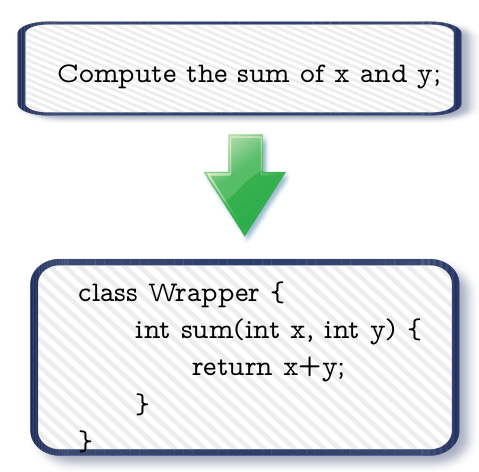
\includegraphics[scale=0.3]{convert.png}
\caption{A simple example of synthsizing the psudo code to its Java implementation}\label{fig:convert}
\end{figure}


\section{Methodology}
We formalize the key idea of our approach through the core language shown in
figure~\ref{fig:language}.

We leverage the KRISP approach(Kate and Mooney, 2006) to model the relation 
between the node in the pseudo code and the element in the target language.

 \begin{figure}[t]
 \small
\[
\begin{array}{lll}
{\rm Program} \ P & := & C^+ \\
{\rm ClassDecl} \ C & := & {\rm class} \ T_1 \ [{\rm extends} \ T_2]? \ \{F^*; M^*\} \\
{\rm FieldDecl}  \ F & := & T \  {\rm fld\_name}; \\
{\rm MethodDecl} \ M & := & m(T_0 \ v_0, \ \ldots, \ T_k \ v_k) = \{ V^*; I; \} \\
{\rm VarDecl} \ V & := & T \  {\rm var\_name}; \\
{\rm Instruction} \ I & := & v_1 = v_2 \ | \ v_1 = v_2.f \ | \ v_1.f = v_2 \\
& & | \ v = {\rm new}^\rho \ T  \ |  \ {\rm if}(*) \ I_1 \ {\rm else} \ I_2 \ | \ I_1; I_2 \\
& & | \ m^\rho@T(v_1, \ldots, v_n) \ | \ v_0.m^\rho(v_1, \ldots, v_n) 
\end{array}
\]
\vspace{-0.2in}
\caption{Core language used for our formalization}\label{fig:language}
\vspace{-0.1in}
\end{figure}

\section{Evaluation and Metrics}

\subsection{Dataset}

Our dataset comes from the following sources: (1) Traditional algorithms 
from textbooks such as TAOCP and CLRS; (2) Mass algorithms from the internet
 such as Stackoverflow and Wikipedia.  

\subsection{Metrics}
To measure the performance of the system, we mainly focus on the precision of
the semantic parse tree. Since if the system can turn the pseudo code into 
its corresponding parse tree in our context free grammar,  we can turn it into 
the implementation through a syntax directed translation. More specifically,
we do the followings: (1) Manually write down actual parse tree and check if
we agree on the output from the system; (2)  Compute the exact match between
the output of the system and the one from human; (3) Compute the F-score for the
parse tree, which gives a partial credit to each outcome.


% include your own bib file like this:
%\bibliographystyle{acl}
%\bibliography{acl2015}

\begin{thebibliography}{}

\bibitem[\protect\citename{Aho and Ullman}1972]{Aho:72}
Alfred~V. Aho and Jeffrey~D. Ullman.
\newblock 1972.
\newblock {\em The Theory of Parsing, Translation and Compiling}, volume~1.
\newblock Prentice-{Hall}, Englewood Cliffs, NJ.

\bibitem[\protect\citename{{American Psychological Association}}1983]{APA:83}
{American Psychological Association}.
\newblock 1983.
\newblock {\em Publications Manual}.
\newblock American Psychological Association, Washington, DC.

\bibitem[\protect\citename{{Association for Computing Machinery}}1983]{ACM:83}
{Association for Computing Machinery}.
\newblock 1983.
\newblock {\em Computing Reviews}, 24(11):503--512.

\bibitem[\protect\citename{Chandra \bgroup et al.\egroup }1981]{Chandra:81}
Ashok~K. Chandra, Dexter~C. Kozen, and Larry~J. Stockmeyer.
\newblock 1981.
\newblock Alternation.
\newblock {\em Journal of the Association for Computing Machinery},
  28(1):114--133.

\bibitem[\protect\citename{Gusfield}1997]{Gusfield:97}
Dan Gusfield.
\newblock 1997.
\newblock {\em Algorithms on Strings, Trees and Sequences}.
\newblock Cambridge University Press, Cambridge, UK.

\end{thebibliography}

\end{document}
